\documentclass{article}

\usepackage{graphicx}
\usepackage{subcaption}
\usepackage{amssymb}
\usepackage[utf8]{inputenc}
\usepackage[T1]{fontenc}
\usepackage[usenames, dvipsnames]{color}
\usepackage{framed}

\renewcommand{\familydefault}{\sfdefault}
\usepackage[scaled=1]{helvet}
\usepackage[helvet]{sfmath}
\everymath={\sf}

\title{Reporte de Actividad 4}

\author{Diego Iván Moreno Campa}

\date{8 de Febrero, 2018}

\begin{document}

\maketitle

\bigskip

\section{Introducción}

Esta actividad es el tercer trabajo para la materia de Física computacional I en la licenciatura de Física.

Los sistemas operativos UNIX y otros sistemas derivados, como lo es Linux y macOS, se apoyan con un intérprete de comandos (Shell), quien es juega el papel de intermediario entre el usuario y el sistema operativo.

Hay toda una familia de intérpretes de comandos para los sistemas operativos. Entre ellos están:  C Shell (/bin/csh), Bourne Shell (/bin/sh), Korn Shell (/bin/ksh/), Bourne Again Shell (/bin/bash), y otros. 

En el caso de la mayoría de las variantes de Linux y macOS, por default viene el intérprete /bin/bash.

En esta actividad, exploraremos las distintas formas de interactuar y hacer programas (scripts) con el Bourne Shell (/bin/sh) y el Bourne Again Shell /bin/bash. En cierta forma en las actividades anteriores, hemos estado haciendo programas (scripts) para los lenguajes interpretados LaTeX y Python.

\section{Fundamentos}

Primero se debe entender que es lo que haremos, con que lo haremos y para que lo haremos. Como observamos en la práctica pasada, el manejo de datos como el que realizamos para la tabla de datos que se descargo de la universidad de Wyoming es algo tedioso si se quiere aplicar a muchos mas datos. Para esto se requiere de automatización de las descargas y el desprecio de los renglones indeseados.
Utilizando el interpretador de Unix Bourne Again Shell podemos automatizar este manejo de archivos creando archivos de script .sh.

Los comandos para la obtención de datos, organización de archivos, herramientas para ver y filtrar contenidos que requerimos para esto son los siguientes:
\begin{itemize}
\item \textbf{cat:} es un comando para leer archivos en una secuencia de argumentos dado, escribiendo su salida en la misma secuencia dada. \textit{cat} viene de con\textit{cat}enar.
\item \textbf{chmod:} es un comando utilizado para reescribir permisos para archivos o carpetas en Unix. el nombre es una abreviación de \textit{change mode}.
\item \textbf{echo:} es un comando de Shell para imprimir elementos en pantalla.
\item \textbf{grep:} el comando grep significa \textit{\textbf{global regular expression print}}, o expresión global de impresión regular.
\item \textbf{less:} este programa de Unix se utiliza para leer texto en la terminal una página a la vez.
\item \textbf{ls:} es un comando para enlistar los archivos y carpetas de un directorio en Unix a través de la terminal.
\item \textbf{wc:} es un comando utilizado para contar el número de renglones, palabras y bytes de un archivo o listado de archivos.
\item \textbf{Redirectores:}
  \begin{itemize}
  \item \textbf{ Pipe ( | ):} es un redirector que se utiliza para atribuirle la salida de un comando como la entrada para otro comando.
  \item \textbf{ Output Redirect (>):} es un redirector que se utiliza para atribuirle pasar la salida a otra parte. El ejemplo más común es la impresión a un archivo utilizando echo: 
  \begin{verbatim}
  	
    $echo "Hello World" > hello.txt
    $cat hello.txt
    Hello World
  \end{verbatim}
  \end{itemize}
\end{itemize}
\section{Procedimiento}

Comenzamos descargando un archivo script1.sh proporcionado por el profesor para descargar la lista de datos de la página de la universidad de Wyoming automáticamente. Después de descargar el archivo y ajustarlo a la estación que deseamos, le configuramos los permisos con chmod 755 script1.sh para poder ejecutarlo y empezar a descargar.

Después de que se completó la descarga podemos utilizar el comando less sounding* para visualizar los 12 archivos una página a la vez dentro de la terminal. Utilizando el comando File podemos ver que tipo de ficheros son los archivos que descargamos.

Continuamos concatenando los 12 archivos descargados en un sólo archivo de texto llamado sondeos.txt utilizando la instrucción:
\begin{verbatim}
	
    cat sounding* > sondeos.txt
\end{verbatim}
la cual redirecciona todos los archivos comenzando con sounding a un nuevo archivo de texto llamado sondeos.txt utilizando el comando cat

Luego de esto, podemos utilizar el comando \textit{egrep} para seleccionar únicamente la información que deseemos del archivo sondeos.txt e imprimirlo en un archivo nuevo llamado df2017.csv
\begin{verbatim}
	
    egrep -v 'PRES|hPa' sondeos.txt | &
    &egrep '723665|Showalter|LIFT|SWEAT|K|Totals &
    &|CAPE|CINS|LFCT|CAPV|Temp|Pres|thick|Precip' > df2017.csv
\end{verbatim}

\begin{figure}[h!]
\centering
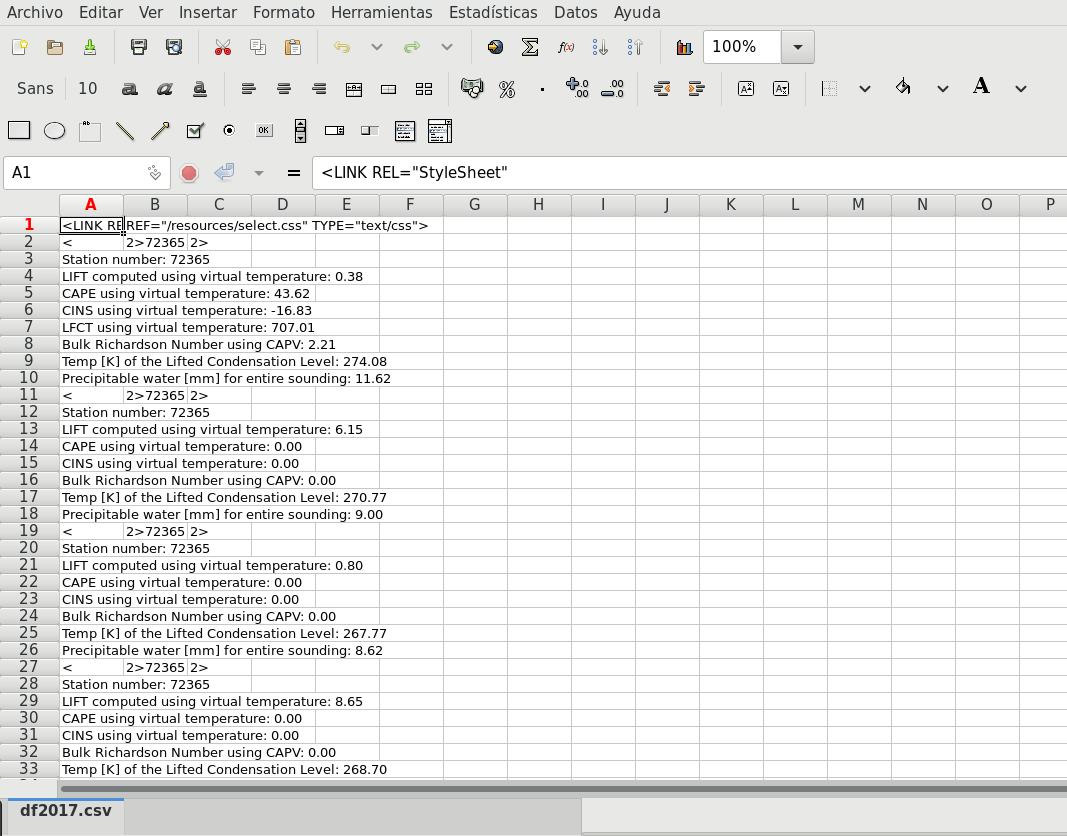
\includegraphics[width=0.5\linewidth]{df2017.png}
\end{figure}

Al observar el archivo notamos que se deshizo de las columnas de datos de presión, temperatura, etc. y se mantuvo únicamente con algunos datos que se mostraban en el pie de página de cada archivo descargado.

Los pasos anteriores también se pueden realizar utilizando un archivo Shell para automatizar el proceso.
Lo llamamos filtro.sh y escribimos las instrucciones utilizadas anteriormente, solamente que ahora los mandamos a un archivo llamado df2017\_2.csv: ~\\

\newpage

\textcolor{red}{script1.sh}
\begin{framed}
\begin{verbatim}
	
    #!/bin/bash
    
    cat sounding* > sondeos.txt
    egrep -v 'PRES|hPa' sondeos.txt | &
    &egrep '723665|Showalter|LIFT|SWEAT|K|Totals|CAPE|CINS&
    &|LFCT|CAPV|Temp|Pres|thick|Precip' > df2017_2.csv
\end{verbatim}
\end{framed}

Después, utilizando el comando \textit{diff} sobre los archivos df2017.csv y df2017\_2.csv no nos señala ninguna diferencia entre los archivos, por lo que el procedimiento es equivalente.

\newpage

\section{Síntesis de Shell Scrpt Tutorial}

\subsection{Introducción}

En esta sección se nos introduce al tutorial, explicando un poco sobre el interpretador Shell, el público al que se dirige y las convenciones de escritura que se utilizarán durante el tutorial.

En las convenciones presentadas se muestra un ejemplo de código para observar el color que se le dara a las cosas durante el tutorial de tal manera que se entienda que es lo que se ve. El ejemplo que se muestra en la página escribe sobre un archivo llamado \textit{myscript.sh}, el cual cambie a \textit{Introduccion.sh}, con el propósito de imprimir \textit{Hello World} a pantalla desde la terminal:

\begin{framed}
\begin{verbatim}
	
    $ echo '#!/bin/sh' > Introduccion.sh
    $ echo 'echo Hello World' >> Introduccion.sh
    $ chmod 755 my-script.sh
    $ ./my-script.sh
    Hello World
    $
\end{verbatim}
\end{framed}

Incluso se muesta que fue lo que produjo el código anterior, que es simplemente el archivo:~\\

\textcolor{red}{Introduccion.sh}
\begin{framed}
\begin{verbatim}
	
    #!/bin/bash
    echo Hello World
\end{verbatim}
\end{framed}

\subsection{Filosofía}

En esta sección el autor describe cuales son las razones por las cuales éste interpretador es mal visto a comparación de otros como Perl o incluso C.

Habla principalmente del hecho de que el código en Shell es fácil de comprender y es más fácil de programar, por lo que se pueden encontrar muchos scripts mal escritos por ahí, menciona también que la indentación crea un problema al leer código en scripts como estos.

Siguiendo con la descripción de lo erroneo con Shell es que hay códigos como el siguiente:
\begin{verbatim}
	
    cat /tmp/myfile | grep "mystring"
\end{verbatim}
correrían más rápido si estuvieran escritos de la siguiente manera:
\begin{verbatim}
	
    grep "mystring" /tmp/myfile
\end{verbatim}
debido a la cantidad de programas y memoria que se utilizan, el interpretador tiene que trabajar más, lo cual en una sola instrucción no es mucho, pero si se desea repetir el proceso una y otra vez se ahorraría bastante tiempo.

\subsection{Un primer Script}

En esta sección se nos reintroduce de manera formal al primer script presentado en introducción, el cual únicamente imprime el texto \textit{Hello World!}, con lo que sigue a mostrar ejemplos de que pasaría si quisieramos poner espacios entre Hello y World, explicando que echo solo deja un espacio entre cada parámetro y por lo que si queremos los espacios debemos poner todo en comillas, como se muestra a continuación:~\\

\textcolor{red}{PrimerScript1.sh}
\begin{framed}
\begin{verbatim}
	
    #!/bin/bash
    # This is a comment!
    echo "Hello      World"       # This is a comment, too!
\end{verbatim}
\end{framed}

Una vez probamos lo anterior se nos presenta un código para observar que espacios pueden ocurrir y cuales no:

~\\
\textcolor{red}{PrimerScript2.sh}
\begin{framed}
\begin{verbatim}
	
    #!/bin/bash
    # This is a comment!
    echo "Hello      World"       # This is a comment, too!
    echo "Hello World"
    echo "Hello * World"
    echo Hello * World
    echo Hello      World
    echo "Hello" World
    echo Hello "     " World
    echo "Hello "*" World"
    echo `hello` world
    echo 'hello' world
\end{verbatim}
\end{framed}
 
 El cual tiene la siguiente salida:
 
\begin{verbatim}
	
    Hello      World
    Hello World
    Hello * World
    Hello * World
    Hello World
    Hello World
    Hello       World
    Hello * World
    world
    hello world
\end{verbatim}

\subsection{Variables - Parte I}

En esta sección se menciona como la mayoría de los lenguajes de programación tienen el concepto de \textit{variables}, un conjunto de espacio en la memoria apartado, el cual también se encuentra en Shell.

Al asignarle un valor a las variables es necesario no dejar espacios alrededor del signo "=". Otra característica de este lenguaje es que no es un lenguaje tipado, lo que significa que a Shell no le importa que hay después del signo con que sea un solo parámetro, por lo que valores "String" deben estar escritos entre comillas:

~\\
\textcolor{red}{VarPI-1.sh}
\begin{framed}
\begin{verbatim}
	
    #!/bin/bash
    MY_MESSAGE="Hello World"
    echo $MY_MESSAGE
\end{verbatim}
\end{framed}

El cual también imprime "\textit{Hello World}", únicamente ahora utilizando una variable.

A diferencia de algunos otros lenguajes, en este no es necesario declararlas previamente, lo que puede causar problemas al tratar de llamar una variable que aun no existe, sólamente se imprimira un espacio. 

~\\
\textcolor{red}{VarPI-2.sh}
\begin{framed}
\begin{verbatim}
	
    #!/bin/bash
    echo "MYVAR is: $MYVAR"
    MYVAR="hi there"
    echo "MYVAR is: $MYVAR"
\end{verbatim}
\end{framed}

Que nos da el siguiente resultado:
\begin{verbatim}
	
    MYVAR is:
    MYVAR is: hi there
\end{verbatim}

Esto ocurre debido a que \textit{MYVAR} no tiene un valor asignado anteriormente a la primera impresión.

Otro equivoco que podria pasar es que queramos concatenar una variable con alguna cadena para crear una nueva variable con simplemente escribir la variable junto a la cadena:
\begin{verbatim}
	
    #!/bin/bash
    echo "What is your name?"
    read USER_NAME
    echo "Hello $USER_NAME"
    echo "I will create you a file called $USER_NAME_file"
    touch $USER_NAME_file
\end{verbatim}

Sin embargo, esto sí es posible solo que utilizando las llaves "{}" sobre el nombre de la variable:

~\\
\textcolor{red}{VarPI-3.sh}
\begin{framed}
\begin{verbatim}
	
    #!/bin/bash
    echo "What is your name?"
    read USER_NAME
    echo "Hello $USER_NAME"
    echo "I will create you a file called ${USER_NAME}_file"
    touch "${USER_NAME}_file"
\end{verbatim}
\end{framed}

De esta forma Shell reconoce donde termina el nombre de la variable, asi logrando concatenar con otra cadena.

\subsection{Comodín}

Utilizar comodines en Unix no es nuevo. Los comodines se utilizan para seleccionar varios archivos que compartan un texto específico o una dirección. Después se especificaran otros usos.

\subsection{Caracteres de escape}

Ciertos caracteres son especiales para Shell, como hemos visto al utilizar \textit{echo} para imprimir una cadena escrita entre ( " ).

La mayoría de los caracteres son tomados literalmente cuando se envuelven en estas ( " ) como ( *, ' , etc.). Sin embargo, los siguientes carcteres ", $\$$, `, and $\backslash$ siguen siendo interpretados por Shell incluso cuando se encuentran entre comillas,
por lo que el carácter $\backslash$ se utiliza para que estos caracteres sean interpretados literalmente dentro de comillas.

Podemos notar que estos caracteres especiales tienen ciertas funciones: las comillas (") se utilizan para preservar espacio, el \$ se utiliza para denotar variables, el $\backslash$ se utiliza para interpretar literalmente los demas caracteres especiales y el backtick ` se discutira más adelante.

\subsection{Búcles}

En la mayoría de los lenguajes se utilizan los búcles para repetir un segmento de código múltiples veces, es por esto que en Bourne Shell existen el \textbf{for} y \textbf{while} el cual no tiene tantas características como otros.

El comando for iteran a través de un listado hasta que éste acabe. el comando for tiene la siguiente estructura:

~\\
\textcolor{red}{Loops1.sh}
\begin{framed}
\begin{verbatim}
	
    #!/bin/bash
    for i in 1 2 3 4 5
    do
    echo "Looping ... number $i"
    done
\end{verbatim}
\end{framed}

con lo que se imprime:
\begin{verbatim}
	
    Looping .... number 1
    Looping .... number 2
    Looping .... number 3
    Looping .... number 4
    Looping .... number 5
\end{verbatim}

Ahora, los \textbf{while} tienen la siguiente estructura:

~\\
\textcolor{red}{Loops2.sh}
\begin{framed}
\begin{verbatim}
	
    #!/bin/bash
    INPUT_STRING=hello
    while [ "$INPUT_STRING" != "bye" ]
    do
    echo "Please type something in (bye to quit)"
    read INPUT_STRING
    echo "You typed: $INPUT_STRING"
    done
\end{verbatim}
\end{framed}

Lo que ocurre en el ejemplo anterior es que lo que se encuentra dentro del \textit{do} se seguira ejecutando hasta que se ingrese la cadena \textit{bye}.
Otra característica del while es que se pueden utilizar los puntos dobles o cólon (:) para terminar el búcle con un Ctrl+C en cualquier momento.

\subsection{Evaluación}

La evaluaciónse utiliza en casi todos los comandos de Shell, sin embargo, es mayormente llamado por la instrucción if... then... else... el cual tiene la siguiente sintaxis:

\begin{verbatim}
if [ ... ]
then
  # if-code
elif [ something_else ]; then
   echo "Something else"
else
  # else-code
fi
\end{verbatim}

Aqui se puede mostrar que el \textit{if [...]} debe ir separado del \textit{then} por un renglón, lo cual también se puede separar con punto y coma (\textbf{;}). Si se desea evaluar más de dos casos se puede utilizar \textit{elif} para añadir casos a la evaluación con if. También hay una forma de escribir la instrucción \textit{if} de una manera más simple, utilizando \&\& y || nos dan una estructura para evaluar.

\newpage

Otra instrucción que utiliza la evaluación es el \textit{while}, en el siguiente ejemplo se puede observar la sintaxis que utiliza.
El siguiente código evalúa el valor ingresado por el usuario hasta que este sea un valor núlo ( de longitud 0 ).

\textcolor{red}{Test1.sh}
\begin{framed}
\begin{verbatim}
	
    #!/bin/bash
    X=0
    while [ -n "$X" ]
    do
    echo "Enter some text (RETURN to quit)"
    read X
    echo "You said: $X"
    done
\end{verbatim}
\end{framed}

\subsection{ \textit{Case} }

La instrucción \textit{Case} nos ahorra el usar muchos if... then... else. Case tiene una sintaxis realmente simple:

\textcolor{red}{Case1.sh}
\begin{framed}
\begin{verbatim}
	
    #!/bin/bash
    echo "Please talk to me ..."
    while :
    do
    	read INPUT_STRING
    	case $INPUT_STRING in
			hello)
            	echo "Hello yourself!"
                ;;
    		bye)
    			echo "See you again!"
    			break
   				;;
    		*)
    			echo "Sorry, I don't understand"
    			;;
    	esac
    done
    echo 
    echo "That's all folks!"
\end{verbatim}
\end{framed}

Como se puede ver, primero evalúa el valor de \$INPUT\_STRING, luego prueba si el valor ingresado concuerda con la opción \textit{hello} o la opción \textit{bye} detras de un paréntesis derecho. Sí esto sucede, corre el bloque de código correspondiente hasta encontrarse con las dobles punto y coma (;;). La tercera opción *) prueba para cualquier otro valor, como se observó en la sección comodín.

\subsection{Variables - Parte II}

Hay un grupo de variables que ya estan disponibles para ti, a las cuales no se les puede asignar un valor.
\begin{itemize}
\item La variable \$0 es el nombre base del programa con el que fue llamado
\item Las variables \$1 al \$9 son los primeros 9 parametros adicionales con los que se llama el programa
\item La variable \$@ contiene todos los parametros del \$1 hasta donde sea.
\item La variable \$\# es el número de parametros con el que fue llamado el programa
\end{itemize}

~\\
\textcolor{red}{VarPII-1.sh}
\begin{framed}
\begin{verbatim}
	
    #!/bin/bash
    echo "I was called with $# parameters"
    echo "My name is $0"
    echo "My first parameter is $1"
    echo "My second parameter is $2"
    echo "All parameters are $@"
\end{verbatim}
\end{framed}

El código anterior muestra el siguiente resultado:
\begin{verbatim}
$ /home/steve/var3.sh
I was called with 0 parameters
My name is /home/steve/var3.sh
My first parameter is
My second parameter is    
All parameters are 
$
$ ./var3.sh hello world earth
I was called with 3 parameters
My name is ./var3.sh
My first parameter is hello
My second parameter is world
All parameters are hello world earth
\end{verbatim}

Otra variable especial es el \$? que contiene el valor de éxito del último comando ejecutado tomando valor 0 si todo salió correctamente y valores diferentes de 0 al encontrar un error, por lo que se puede utilizar para la detección de errores.

Y las otras variables especiales \$\$ y \$! son números de proceso. La variable \$\$ es un identificador para el proceso actual mientras que la variable \$! es un identificador del proceso anterior.

Por último, otra variable interesante es el IFS, abreviación de \textit{Internal Field Separator} que significa separador de campo interno, el cual se utiliza para que Shell interprete su valor como el separador al leer datos. El valor predeterminado de IFS es el espacio, tabulación y salto de línea. Este se puede utilizar de la siguiente manera:

~\\
\textcolor{red}{VarPII-2.sh}
\begin{framed}
\begin{verbatim}
	
    #!/bin/bash
    old_IFS="$IFS"
    IFS=:
    echo "Please input some data separated by colons ..."
    read x y z
    IFS=$old_IFS
    echo "x is $x y is $y z is $z"
\end{verbatim}
\end{framed}

\subsection{Variables - Parte III}

Para las variables, podemos utilizar las llaves {} entre el nombre para concatenar con otro segmento de texto y crear una nueva variable. Las llaves son útiles para lidiar con variables indefinidas o sin valor.

La herramienta de Shell ":-" se utiliza dentro de unas llaves para especificar un valor predeterminado para una variable sin valor, mientras que el signo ":=" se utiliza de la misma manera para especificar un valor predeterminado para una variable indefinida.

\subsection{Programas externos}

En Shell se utilizan mucho los programas externos, como lo son \textit{tr}, \textit{grep} y \textit{expr}. El backtick (`) está asociado a los comandos externos la mayoría del tiempo, el cual se utiliza para indicar que el texto encerrado se ejecutara como comando. Ésto es muy útil para ahorrar memoria para procesos lentos como en el siguiente ejemplo:

~\\
\textcolor{red}{ExtProg1.sh}
\begin{framed}
\begin{verbatim}
	
    #!/bin/bash
    HTML_FILES=`find / -name "*.html" -print`
    echo "$HTML_FILES" | grep "/index.html$"
    echo "$HTML_FILES" | grep "/contents.html$"
\end{verbatim}
\end{framed}

La variable \textit{HTML\_FILES} que utiliza un comando lento \textit{find} solamente se llama una vez, en lugar de las dos veces que se utilizó, así acortando el tiempo de ejecución por alrededor de la mitad.

\subsection{Funciones}

En Shell se pueden crear facilmente funciones que inicialmente se leen, y se corren hasta que son explicitamente llamadas, sólo que estas no son recursivas como en otros lenguajes. Cuando se tiene un paquete de funciones, estas se pueden declarar llamando una libreria que las contenga de varias maneras, una de ellas es la siguiente:
\begin{verbatim}
. ./library.sh
\end{verbatim}

Una función se declara utilizando al final de su nombre "()" y encerrando su código en llaves "{}" como se muestra en el ejemplo:

~\\
\textcolor{red}{Func1.sh}
\begin{framed}
\begin{verbatim}

	#!/bin/bash
    # A simple script with a function...
    
    add_a_user()
    {
    	USER=$1
        PASSWORD=$2
        shift; shift;
        # Having shifted twice, the rest is now comments ...
        COMMENTS=$@
        echo "Adding user $USER ..."
        echo useradd -c "$COMMENTS" $USER
        echo passwd $USER $PASSWORD
        echo "Added user $USER ($COMMENTS) with pass $PASSWORD"
    }
    
    ###
    # Main body of script starts here
    ###
    echo "Start of script..."
    add_a_user bob letmein Bob Holness the presenter
    add_a_user fred badpassword Fred Durst the singer
    add_a_user bilko worsepassword Sgt. Bilko the role model
    echo "End of script..."
\end{verbatim}
\end{framed}
ba
De este ejemplo se nota que las funciones hacen uso de parametros al ser llamados al igual que al llamar un programa. Los parametros con los que son llamados las funciones son internos para el instante en el que se llamaron. Sin embargo, las variables modificadas dentro de una función toman valores globales como se muestra en el siguiente ejemplo:

~\\
\textcolor{red}{Func2.sh}
\begin{framed}
\begin{verbatim}
	
    #!/bin/bash
    
    myfunc()
    {
    	echo "I was called as : $@"
        x=2	
    }
    
    ### Main script starts here 
    
    echo "Script was called with $@"
    x=1
    echo "x is $x"
    myfunc 1 2 3
    echo "x is $x"
\end{verbatim}
\end{framed}

que tiene como salida lo siguiente utilizando como parametros a b c; se puede notar que el valor de \textit{X} no se preservó una vez se regresó al código principal:

\begin{verbatim}
Script was called with a b c
x is 1
I was called as : 1 2 3
x is 2
\end{verbatim}

Para crear una librería simplemente se crea un archivo .lib, este no necesita contener un \textit{\#!/bin/bash} debido a que sera llamado en un archivo Shell, donde ya habrá sido establecido.
Después, únicamente para llamarlo se utiliza el programa "." de la siguiente manera:
En este caso, la librería se llama \textit{common.lib}

\begin{verbatim}
#!/bin/bash
# function2.sh
. ./common.lib
echo $STD_MSG
rename .txt .bak
\end{verbatim}

\subsection{Pistas y Consejos}

Unix esta lleno de herramientas para el manejo de texto. La significancia de esto, es el hecho de que virtualmente todo debajo de Unix es texto. Virtualmente todo lo que se puede pensar es controlado ya sea por archivos de texto o por una iterface de línea-comando (CLI). La única cosa que no se puede automatizar usando scripts de Shell es una herramienta de sólo Interface gráfica de usuario. Y bajo Unix, no hay muchas de ellas.

\newpage

\section{Bibliografía}
\begin{itemize}
\item Steve Parker (2017). Shell Script Tutorial (https://www.shellscript.sh/)
\item thoughtbot, inc. (2018). Input/Output Redirection in the Shell. (https://robots.thoughtbot.com/input-output-redirection-in-the-shell)
\end{itemize}

\newpage

\title{Apéndice}

\begin{enumerate}
\item ¿Qué fue lo que más te llamó la atención en esta actividad? ~\\~\\
El uso del interpretador de lenguaje de máquina para Unix para la automatización de manejo de archivos por nuestra propia cuenta.

\item ¿Qué consideras que aprendiste? ~\\~\\
A manejar un poco el interpretador Shell como algunas herramientas para cortar, leer, concatenar y reemplazar lineas de texto para algunos archivos.

\item ¿Cuáles fueron las cosas que más se te dificultaron? ~\\~\\
Realizar la síntesis del tutorial se me dificultó porque no podía dejar pasar cosas que no conocía, así que me termino tomando bastante tiempo para comprender todo y poder escribir lo que entendí.

\item ¿Cómo se podría mejorar en esta actividad? ~\\~\\
La práctica esta bien

\item ¿En general, cómo te sentiste al realizar en esta actividad? ~\\~\\
Me sentí bien al realizar la práctica, excepto al momento de escribir la síntesis como dije anteriormente

\end{enumerate}

\end{document}
